\documentclass[a4paper]{report}
\usepackage[utf8]{inputenc}
\usepackage[T1]{fontenc}
\usepackage{RJournal}
%\usepackage{amsmath,amssymb,array}
\usepackage{array}
\usepackage{booktabs}

%\usepackage{natbib}
\usepackage[cmex10]{amsmath}
\usepackage{amsfonts,amssymb,amsthm}
%\usepackage{rotating}
%\usepackage{multirow}
%\usepackage{graphicx}
%\usepackage{epstopdf}
%\usepackage[draft]{fixme}

%\usepackage{mdwmath}
%\usepackage{mdwtab}
%\usepackage[lined,boxed,commentsnumbered]{algorithm2e}
%\usepackage[misc,geometry]{ifsym}

\usepackage{subcaption}
\theoremstyle{definition}
%\newtheorem{example}{Example}[section]


\newcommand{\nc}{\newcommand}

\newcommand{\bmZ}{\mathbf{Z}}
\newcommand{\bmz}{\mathbf{z}}
\newcommand{\bmY}{\mathbf{Y}}
\newcommand{\bmy}{\mathbf{y}}
\newcommand{\bmX}{\mathbf{X}}
\newcommand{\bmx}{\mathbf{x}}
\newcommand{\calQ}{\mbox{$\cal{Q}$}} 
\newcommand{\iprod}[2]{\ensuremath{\langle #1,#2\rangle}}
\newcommand{\bmtheta}{{\mbox{\bm $\theta$}}}
\nc{\bm}{\boldmath}
\newcommand{\TRUEparam}{\ensuremath{\bmtheta^k}}
\nc{\ld}{,\ldots,} \nc{\defi}{:=} \nc{\incl}{\subset}
\nc{\given}{|}
\nc{\KL}[2]{D\left(\,#1\,\norm\,#2\,\right)}
\nc{\norm}{\|} \nc{\sizeof}[1]{\left|#1\right|}
\newcommand{\trans}{^{\mathsf{T}}}

%% load any required packages FOLLOWING this line

\begin{document}

%% do not edit, for illustration only
\sectionhead{Contributed research article}
\volume{12}
\volnumber{2}
\year{2020}
\month{December}
\setcounter{page}{342}

%% replace RJtemplate with your article
\begin{article}
  % !TEX root =  RJwrapper.tex
\title{\pkg{MoTBFs}: An R Package for Learning Hybrid Bayesian Networks Using Mixtures of Truncated Basis Functions}
\author{by Inmaculada Pérez-Bernabé, Ana D. Maldonado, Antonio Salmerón and Thomas D.\ Nielsen}

\maketitle

\abstract{
This paper introduces  \CRANpkg{MoTBFs}, an R package for manipulating  
mixtures of truncated basis functions. This class of functions allows the representation of
joint probability distributions involving discrete and continuous variables simultaneously, and
includes mixtures of truncated exponentials and mixtures of polynomials as special cases.
The package implements functions for learning the parameters of univariate, multivariate, and conditional
distributions, and provides support for parameter learning in Bayesian networks with
both discrete  and continuous variables. Probabilistic inference using forward sampling is also implemented.
Part of the functionality of the \pkg{MoTBFs} package relies on the \CRANpkg{bnlearn} package, which includes
functions for learning the structure of a Bayesian network from a data set. Leveraging this functionality, the \pkg{MoTBFs}
package supports learning of MoTBF-based Bayesian networks over hybrid domains. 
We give a brief introduction to the methodological context and algorithms implemented in the package.
An extensive illustrative example is used to describe the package, its functionality, and its usage.
}

\section{Introduction}

Mixtures of truncated basis functions (MoTBFs) \citep{Lan12} have  been proposed as a
general framework for handling hybrid Bayesian networks, i.e., Bayesian networks where discrete
and continuous variables coexist. As special cases, the framework includes the so-called mixtures of truncated exponentials
(MTEs) \citep{Mor01} and mixtures of polynomials (MoPs) \citep{She11,LoCru12}.

One of the advantages of MoTBFs is that they allow for hybrid Bayesian networks with
no structural restrictions on the relations between the continuous and discrete variables; this is in contrast
to conditional Gaussian (CG) models~\citep{Lau92}, where discrete variables are not 
allowed to have continuous parents. Restricting arc directions is problematic, for instance in situations where the
network structure is given a causal interpretation; the fact that MoTBFs have no such restriction make
them suitable for this kind of analysis. Furthermore, MoTBFs are closed under addition, multiplication, and integration,
which facilitates the use of exact probabilistic inference methods like the Shenoy-Shafer architecture \citep{She90} or
the variable elimination algorithm \citep{Zha96}.

Methods for learning MoTBFs from data have previously been studied and cover algorithms for learning both
marginal~\citep{Lan12b,Lan12} and conditional MoTBF densities from data~\citep{Lan09,Lan14,Per15b}. 
To address situations where data availability is limited, \cite{Per15} proposed a methodology for integrating prior
knowledge when  learning univariate and conditional MoTBFs from data. The underlying idea of the
integration is to represent the prior knowledge as an
MoTBF density that is later combined with the density learned from data, thus resulting in a new MoTBF density.
Together, the learning algorithms for MoTBF-based Bayesian networks facilitate learning in data-rich domains as well as domains where
limited quantitative data is counterbalanced by qualitative domain knowledge.  

The aim of the \pkg{MoTBFs} package is to provide a free and accessible implementation of algorithms for learning
MoTBFs from data. The package implements state-of-the-art learning algorithms for univariate, conditional, and joint MoTBF
densities. By extension, functionality is also provided for learning MoTBF-based Bayesian networks by leveraging 
functionality from the \pkg{bnlearn} package~\citep{Scu10}. Hybrid Bayesian networks supported by \pkg{bnlearn}
are restricted to CG models, which implies that conditional distributions of discrete variables given continuous ones
are not permitted. Other packages like \CRANpkg{deal}~\citep{Boe03} and \CRANpkg{pcalg}~\citep{Kal12}
are also restricted to CG models. By adopting the MoTBF framework, the  \pkg{MoTBFs} package sidesteps this restriction
on the possible network structures.
Furthermore, the \pkg{MoTBFs} package also provides methods for integrating prior
domain knowledge in the learning process, thus also supporting data sparse domains. 

Another package that includes hybrid Bayesian networks functionality is \CRANpkg{HydeNet}~\citep{Dal19}.
This package is able to handle conditional distributions beyond the Gaussian model class, 
but discrete variables conditional on continuous ones are modeled using generalized linear models,
and inference is only possible using Markov Chain Monte Carlo through an interface to JAGS~\citep{Plu03}.
Unlike \pkg{MoTBFs} and \pkg{bnlearn}, \pkg{HydeNet} does not provide functionality for learning the
network structure. \pkg{HydeNet} is especially appropriate for modeling decision problems, since it
implements influence diagrams, which are extensions of Bayesian networks that include decision and utility nodes,
similarly to decision trees.
 
The package  \pkg{abn}~\citep{Kra19} deals with so-called \emph{additive Bayesian networks}, which are
Bayesian networks where each node holds a generalized linear model, and the effect of the parents of each node is
additive in terms of the exponential family expression of the conditional distribution. Unlike \pkg{HydeNet},
\CRANpkg{abn} is able to learn the network structure from data, and adopts a fully Bayesian approach, thus allowing the
specification of prior distributions on the parameters in a natural way. The main difference with respect to
package \pkg{MoTBFs} is that MoTBF distributions do not belong to the exponential family, and in that sense both
packages are complementary. 

%The rest of the paper is organized as follows. Section~\ref{sec:motbf} provides a description of the MoTBF framework.
%The \pkg{MoTBFs} package is presented in Section~\ref{sec:package} along with an illustrative example.
%The paper ends with conclusions in Section~\ref{sec:conclusions}.

\section{Mixtures of truncated basis functions}\label{sec:motbf}

The MoTBF framework \citep{Lan12} is based on the abstract notion of real-valued \emph{basis functions}, 
which includes both polynomial and exponential functions as special cases.

More formally, let $\bmX$ be a mixed $n$-dimensional random vector. Let $\bmY
= (Y_1,\ldots,Y_d)$ and $\mathbf{Z} = (Z_1,\ldots,Z_c)$ be the
discrete and continuous parts of $\bmX$, respectively, with $c
+ d = n$.  Let $\Psi=\{\psi_i(\cdot)\}_{i=0}^{\infty}$ with
$\psi_i:\mathbb{R}\to \mathbb{R}$ define a collection of real basis functions. We say that a function $\hat f:\Omega_{\mathbf{X}}\mapsto
\mathbb{R}_0^+$ is a \emph{mixture of truncated basis functions}\/ potential to level $k$ wrt.\ $\Psi$ 
if  one of the following two conditions holds:

\begin{itemize}
	\item $f$ can be written as
      
	\begin{equation}\label{equ:motbfCore}
	f(\bmx) = f(\bmy,\bmz) =  \sum_{i=0}^k     \prod_{j=1}^c a_{i,\bmy}^{(j)}\, \psi_i\left( z_j \right), 
	\end{equation}
	where $a_{i,\bmy}^{(j)}$ are real numbers. 

	\item There is a partition $\Omega_{\bmX}^1,\ldots,\Omega_{\bmX}^m$ of $\Omega_{\bmX}$ for which   the domain of the continuous variables, $\Omega_{\mathbf{Z}}$, is
	divided into hyper-cubes and such that $f$ is defined as
	$$
	f(\bmx) = f_\ell(\bmx) \quad \mathrm{if}~~ \bmx \in \Omega_{\bmX}^\ell,
	$$
	\noindent
	where each $f_\ell$, $\ell=1,\ldots,m$ can be written in the
	form of Equation~\ref{equ:motbfCore}.
\end{itemize}
Typically, a univariate MoTBF for a variable $X$ does not rely on a partitioning of $\Omega_X$. 

To see the relationship between MoTBFs and MoPs \citep{She11}, we can instantiate the  basis functions as polynomials (i.e.,
$\psi_i(x)=x^i$, for $i=0,\ldots,k$) in which case the MoTBF model reduces to an MoP model. For
example, with polynomial basis functions, a univariate MoTBF of level $k$ for a variable $X$ is given by
\[
f(x) =   \sum_{i=0}^k \theta_{i}\, \psi_i\left( x \right).
\]
Similarly, by having exponential basis functions the MoTBF model implements an MTE model \citep{Mor01}. 
For ease of exposition, we shall in the remainder of this paper assume polynomial basis functions unless
explicitly stated otherwise.



An MoTBF potential is a \emph{density}\/  if  $\sum_{\bmy\in \Omega_{\bmY}} \int_{\Omega_{\bmz}}
f(\bmy,\bmz) d\bmz = 1$. Similarly, we say that an MoTBF $f(\bmy,\bmz)$ is a \emph{conditional density} for
$\bmZ'\subseteq \bmZ$ and $\bmY'\subseteq \bmY$ given $(\bmZ\setminus \bmZ')$ and $(\bmY\setminus \bmY')$ if  
\[
\sum_{\bmy'\in \Omega_{\bmY'}} \int_{\Omega_{\bmz'}}
f(\bmy',\bmy'',\bmz',\bmz') d\bmz' = 1,
\]
for all $\bmz''\in \Omega_{\bmZ\setminus \bmZ'}$ and $\bmy''\in
\Omega_{\bmY\setminus \bmY'}$. Following \cite{Lan12} we furthermore assume that the influence that a set of continuous 
parent variables $\bmZ$ have on their child variable $X$ is encoded only through the partitioning of $\Omega_{\bmZ}$ into 
hyper-cubes, and not directly in the functional form of $f(x\given \bmz)$ inside the hyper-cube $\Omega_{\bmZ}^j$. 
That is, for a partitioning ${\cal P}=\{\Omega_{\boldsymbol{Z}}^1, \ldots, \Omega_{\boldsymbol{Z}}^m\}$ of
$\Omega_{\boldsymbol{Z}}$, the conditional MoTBF
is defined for $ \bmz\in\Omega_{\boldsymbol{Z}}^j$, $1\leq j\leq m$, as
\begin{equation}
\label{equ:conditional_motbf}
f^{(j)}_k(x | \bmz\in \Omega_{\boldsymbol{Z}}^j) =  \sum_{i=0}^k    \theta_{i}^{(j)}\, \psi_i^{(j)}(x).   
\end{equation}
In the remainder of this paper we shall assume that a conditional MoTBF density includes only a single `head'
variable, i.e., $|\bmZ'\cup\bmY'|=1$.  


\subsection{Learning univariate MoTBFs from data}
\label{sec:learningUnivariateMOP}



\citet{Lan14} present a method for learning univariate MoTBF distributions from data. This method is also implemented
in the \pkg{MoTBFs} package and is briefly described here together with its extension to both conditional and
joint distributions.
The estimation procedure relies on the empirical cumulative distribution
function (CDF) as a representation of the data, which, for a sample $D=\{ x_1,\ldots,x_N \}$, is defined as
\begin{equation}
\label{e}
G_N(x) = \frac{1}{N} \sum_{\ell=1}^N \mathbf{1}\{ x_\ell\leq x\}, \quad x\in \mathbb{R},
\end{equation}
where $\mathbf{1}\{ \cdot \}$ is the indicator function. 

The algorithm developed by \cite{Lan14} fits a potential, whose derivative is an MoTBF, to the empirical CDF using least squares.
As an example, if we use polynomials as basis functions, 
$\Psi=\{1, x, x^2,x^3,\ldots\}$, the parameters of the CDF, denoted as $c_0,\ldots,c_k$, are estimated by solving 
the optimization problem
\begin{align}
\underset{c_0,\ldots,c_k}{\mathbf{minimize}} & \displaystyle  \sum_{\ell=1}^N \left(G_N(x_\ell) - \sum_{i=0}^{k} c_{i}\,x_\ell^i\right) ^2  \notag  \\
\mathbf{subject~to} & \displaystyle \sum_{i=1}^{k} i \,c_{i}\,x^{i-1} \geq 0  \quad \forall x\in \Omega ,  \label{eq:program_MOP}\\
& \displaystyle \sum_{i=0}^{k} c_{i}\,\alpha^i =0 \notag 
\text{ and }    \notag 
\displaystyle \sum_{i=0}^{k} c_{i}\,\beta^i =1,  \notag
\end{align}
where the constraints ensure that the obtained parameter estimates define a valid CDF, with $\alpha$ and $\beta$ being
the minimum and maximum values of the data sample, respectively. More precisely, the first constraint guarantees that
the corresponding density is non-negative and the last two restrictions ensure that it integrates to 1. The
latter is 
equivalent to stating that the CDF should be equal to 0 at the minimum and equal to 1 at the maximum.
Note that the estimated function is not actually a density, but a  CDF instead. An MoTBF density can be
obtained by simply taking the derivative of the CDF.

Note that the optimization program above is convex, and can be efficiently solved in theory. However, the infinite 
number of constraints introduced by imposing that $\frac{{\rm d} F(x)}{{\rm d}x} \geq 0$ for {\em all} $x\in \Omega_X$ 
complicates the implementation on a computer. In practice, we only check that the constraint is fulfilled for a limited set of 
points spread across $\Omega_X$.

In learning scenarios involving a  large amount of data (i.e., when $N$ is large), solving the program can be time 
consuming. In such cases we  define a {\em grid} on $\Omega_X$, that is selected so that the number of observations 
is the same between each pair of consecutive grid-points. The grid-points are used to evaluate the objective function
instead of the sample points. 

The level $k$ of the estimated MoP can be decided using different model selection techniques. 
For the results presented in this paper we have performed a greedy search, choosing the value for $k$
maximizing the Bayesian information criterion (BIC) \citep{Sch78}:
\begin{equation}
\label{eq:bic}
\text{BIC}(f,D) = \sum_{\ell=1}^N \log f(x_\ell) - \frac{k+2}{2} \log N.
\end{equation}

This choice is motivated by \cite{Lan14}, who showed that the estimators based on Equation \ref{eq:program_MOP} are consistent  in terms of the mean squared error for all $x\in \Omega_X$.


\subsection{Learning conditional MoTBFs from data}
\label{sec:learningConditionalMOP}
In a conditional MoTBF density, the continuous parent variables $\bmZ$ only influence the child variable $X$
through the partitioning of the domain of $\bmZ$ into hyper-cubes, and not directly in the functional form of $f(x | \bmz)$ inside each
hyper-cube \citep{Lan12}. Thus, learning a conditional MoTBF basically consists in finding a partitioning of the
domain of the parent variables and using the procedure above for estimating the density of the child variable
for each of these partitions.

This procedure is formally described by  \cite{Lan14}, where the domain of the parent variables,
$\Omega_{\bmZ}$, is incrementally split as long as the BIC score
improves. Equal frequency binning is used to determine candidate split points. After splitting a variable $Z$, 
the algorithm fits a univariate MoTBF density for each induced sub-partition $\Omega_{\boldsymbol{Z}}^{1}$ and
$\Omega_{\boldsymbol{Z}}^{2}$. A candidate partition $\Omega_{\boldsymbol{Z}'}$ is only accepted 
if the BIC score is improved, i.e., if 
\[
\text{BIC-Gain}(\Omega_{\boldsymbol{Z}}',Z) = \text{BIC}(f',D) - \text{BIC}(f,D) > 0,
\]
where $f'$ is the conditional MoTBF potential defined over the candidate partition.




\subsection{Learning joint MoTBFs from data}
\label{sec:learningJointMOP}

The procedure for learning joint densities is an extension of the  program in Equation \ref{eq:program_MOP} to random vectors of
arbitrary dimension \citep{Per15b}. 
In the multivariate case, the sample is a set of $d$-dimensional observations, 
${\cal D}=\{ \bmx_1,\ldots,\bmx_N \}$, $\bmx\in\Omega_\bmX\subset\mathbb{R}^d$. 
We say that the event $\bmx_\ell \leq \bmx$ is true if and only if $\bmx_{\ell,i} \leq \bmx_i$ for each dimension $i=1,\ldots, d$.
For notational convenience we use $\Omega_\bmX^-\in\mathbb{R}^d$ to denote the minimal point of $\Omega_\bmX$ (obtained by choosing the minimum of $\Omega_\bmX$ in each dimension), and let $\Omega_\bmX^+\in\mathbb{R}^d$ be the corresponding  maximal point. Then, the empirical CDF is defined as
\begin{equation}
\nonumber
G_N(\bmx) = \frac{1}{N} \sum_{\ell=1}^N  \mathbf{1}\{ \bmx_\ell\leq \bmx\}, \quad \bmx \in  \Omega_\bmX\subset\mathbb{R}^d.
\end{equation}
The goal is to find a representation of the empirical CDF of the form 
$$F(\bmx)=\sum_{\ell_1=0}^k \ldots \sum_{\ell_d=0}^k c_{\ell_1,\ell_2,\ldots,\ell_d} \prod_{i=1}^d x_i^{\ell_i},$$
obtained by solving the optimization problem
\begin{align}
\mathbf{minimize} & \displaystyle  \sum_{\ell=1}^N \left(G_N(\bmx_\ell) - F(\bmx_\ell)\right) ^2  \notag  \\
\mathbf{subject~to} & ~~\displaystyle \frac{\partial^d F(\bmx)}
{\partial x_1, \dots, \partial x_d} \geq 0  \quad \forall \bmx \in \Omega_\bmX,\label{eq:jointN_MOP}\\
& 
\displaystyle F\left(\Omega_\bmX^-\right) =0 \notag  \text{ and }    \notag  \displaystyle F\left(\Omega_\bmX^+\right) =1.  \notag
\end{align}


The solution to this problem is the parameter-set that defines the joint CDF, and the density can be obtained 
by differentiation of the joint CDF.  As in the univariate case, it is a quadratic optimization problem, 
that can be solved efficiently if the objective function is only evaluated on a set of grid-points.


\subsection{Incorporating prior knowledge}\label{sec:priorKnowledge}
\label{sec:incorporatingKnowledge}

There are real world situations, where the amount of available data is insufficient for 
accurate density estimation. The \pkg{MoTBFs} package includes implementations oriented
to face these kinds of situations by allowing prior knowledge to be taken into account during density estimation.
In Bayesian statistics~\citep{Ber09}, prior information is encoded as prior probability distributions over the parameters. 
As an example, consider the case of a random variable representing the body temperature of a patient in a hospital,
and assume that the variable is normally distributed with mean $\mu$ and standard deviation $\sigma$. Prior knowledge could 
be provided in the form of a prior distribution on $\mu$ by establishing that $\mu \sim {\cal N}(37,0.1)$.
However, in the case of MoTBF distributions, the parameters do not have a meaning in general. Therefore, 
there is no clear way in which a practitioner could provide prior information on any of the parameters,
although some 
information could still be specified. For instance, in the body temperature example, the practitioner could choose not to give 
prior information on any single parameter,  but instead provide a full distribution of the variable, reflecting
his or her prior knowledge when no data is available. Such prior information could, e.g., include that the body temperature follows  
a normal distribution with mean 37 and standard deviation 0.5. This is the approach followed by \cite{Per15}, where prior
knowledge is encoded as an MoTBF distribution over the random variable, which is then later combined
with the MoTBF density learned from data.  

In order to represent such a prior distribution as an MoTBF, a sample is drawn from the prior -- e.g., ${\cal N}(37,0.1)$
in the example above -- and the sample is then used to learn an MoTBF using the methods previously described in
this paper. Alternatively, one may also rely on direct translation schemes as described in, e.g., \citep{Lan10,Cob06}.   

Given a prior MoTBF density $f_{\emph{prior}}$ over a variable $X$, \cite{Per15} obtain a posterior density
$f_{\emph{post}}$ by making a linear
combination of the prior density and the density $f_{\emph{data}}$ learned from data, expressed as
\[
f_{\emph{post}}  = w_{p} f_{\emph{prior}} + w_{d} f_{\emph{data}}\ \ , 
\]
where $w_{p}$ is the weight of $f_{prior}$ and $w_{d}$ is the weight of $f_{data}$, with 
$0\leq w_{p} \leq 1$, $0\leq w_{d} \leq 1$ and $w_p+w_d=1$. The weights $w_p$ and $w_d$ 
reflect the way in which they explain the observed data. They are computed by measuring the difference between the
log-likelihood produced by each one of the densities ($f_{\emph{prior}}$ and $f_{\emph{data}}$) and 
the expected log-likelihood that would be produced by a randomly generated MoTBF.
See \citep{Per15} for a detailed explanation of the procedure.


\subsection{Probabilistic inference}
\label{sec:inference}

In a Bayesian network, probabilistic inference is the task of computing the posterior distribution of any
variable $X$  given that some other variables $\bmY$ have been
observed to take some value $\bmy$. Therefore, the goal of probabilistic inference is to compute
the density $f(x|\bmy)$, where the value $\bmy$ is fixed. 

An easy approach to estimate this density is by \emph{forward sampling}~\citep{Hen88}.
The idea is to draw a sample of configurations of the variables in the Bayesian network by simulating each variable
using its conditional distribution following a top-down order. Prior to sampling, all the densities
in the network are restricted to the value $\bmY=\bmy$ and when a variable is to be sampled,
its conditional distribution is restricted to the values already obtained for its parents. 
Sampling is always possible since the variables are sampled following the topological ordering of the network.
Once the sample has been obtained,
$f(x|\bmy)$ is estimated as a univariate MoTBF as we described before. 


\section{Package description and illustrative example} \label{sec:package}

The \pkg{MoTBFs} package  is designed using \code{S3} objects.
The functions provided by the package
implement the methods explained in the previous sections.
The package implements functions for learning univariate, multidimensional, and
conditional distributions, and provides support for parameter learning in  hybrid Bayesian
networks. In addition, it includes functions for incorporating prior knowledge when 
there is lack of data and for carrying out probabilistic inference.
Moreover, two classes are incorporated in the package, \code{"motbf"} for defining univariate mixtures of truncated basis functions 
and \code{"jointmotbf"} for specifying multidimensional MoTBFs.

The functionality of the \pkg{MoTBFs} package is illustrated through an analysis carried out on a real world dataset. 
More precisely, we use the \code{ecoli} dataset \citep{Lichman:2013}, which is provided along with the package. 
The dataset contains information about 
\textit{Escherichia coli} and consists of $n = 336$ records, $8$ input variables, and $1$ output variable (the class).  It is a bacterium of the genus \textit{Escherichia} that is commonly found in the lower intestine of warm-blooded organisms.
This dataset can be downloaded from \url{http://archive.ics.uci.edu/ml/datasets/Ecoli}.

To begin the analysis, the package and the data are loaded by

\begin{example}
> install.packages("MoTBFs")
> library("MoTBFs")
> data("ecoli", package = "MoTBFs")
> str(ecoli)

'data.frame':	336 obs. of  9 variables:
$ Sequence.Name: chr  "AAT_ECOLI" "ACEA_ECOLI" "ACEK_ECOLI" "ACKA_ECOLI" ...
$ mcg          : num  0.49 0.07 0.56 0.59 0.23 0.67 0.29 0.21 0.2 0.42 ...
$ gvh          : num  0.29 0.4 0.4 0.49 0.32 0.39 0.28 0.34 0.44 0.4 ...
$ lip          : chr  "0.48" "0.48" "0.48" "0.48" ...
$ chg          : chr  "0.5" "0.5" "0.5" "0.5" ...
$ aac          : num  0.56 0.54 0.49 0.52 0.55 0.36 0.44 0.51 0.46 0.56 ...
$ alm1         : num  0.24 0.35 0.37 0.45 0.25 0.38 0.23 0.28 0.51 0.18 ...
$ alm2         : num  0.35 0.44 0.46 0.36 0.35 0.46 0.34 0.39 0.57 0.3 ...
$ class        : chr  "cp" "cp" "cp" "cp" ...
\end{example}

The \code{ecoli} dataset is a data frame with $336$ rows corresponding to proteins and $9$ columns corresponding to variables.
The dataset contains $4$ discrete variables, stored as characters, and $5$ continuous variables. The variables
provide measurements of the cells used for predicting the localization site of proteins. 
The first variable, \code{Sequence.Name}, which
is the accession number for the SWISS-PROT database, and the output variable \code{class} will not be used
in this running example, and we will  therefore remove them from the data frame.
The discrete variables \code{lip} and \code{chg} are binary attributes, where character numbers are used as states; \code{"0.48"} and \code{"1"}, and \code{"0.5"} and \code{"1"}, respectively. For validation purposes, the dataset is split into 
a training and a test set. 


\begin{example}
>   data <- ecoli[,-c(1,9)]
>   set.seed(2)
>   dataTT <- TrainingandTestData(data, percentage_test = 0.2)
>   trainingData <- dataTT$Training
>   testData <- dataTT$Test
\end{example}

The seed value determines the partitioning of the data into training and test, and is therefore key to
reproducing the experiments.
From now on, we will carry out all the analyses on the training data, leaving the test dataset for estimating the 
predictive capabilities of the learned models.

Our illustrative example basically consists of fitting MoTBF densities to a previously learned Bayesian
network structure over the variables in the dataset. The structure can, for instance, be obtained, using the function \code{hc()}
from the 
\pkg{bnlearn} package. This function returns a directed acyclic graph obtained from the dataset using 
a local search method. For the sake of simplicity, we have included the function \code{LearningHC()} in our package,
which automatically converts into factors those columns that are non-numeric, before calling the function \code{hc()}
in \pkg{bnlearn}.  \code{LearningHC()} can also be used to discretize the dataset before calling \code{hc()}, but
we are not using this functionality in the running example.

\begin{example}
>   dag <- LearningHC(trainingData)
>   dag

Bayesian network learned via Score-based methods

model:
[lip][alm1][mcg|lip:alm1][chg|lip][aac|alm1][gvh|mcg][alm2|gvh:lip:alm1] 
nodes:                                 7 
arcs:                                  8 
undirected arcs:                       0 
directed arcs:                         8 
average markov blanket size:           3.14 
average neighbourhood size:            2.29 
average branching factor:              1.14 

learning algorithm:                    Hill-Climbing 
score:                                 BIC (cond. Gauss.) 
penalization coefficient:              2.797356 
tests used in the learning procedure:  102 
optimized:                             TRUE 
\end{example}

\begin{example}
> plot(dag)
\end{example}


The network structure obtained is shown in Figure~\ref{fig:dag}. 

\begin{figure}[htbp]
	\centering

	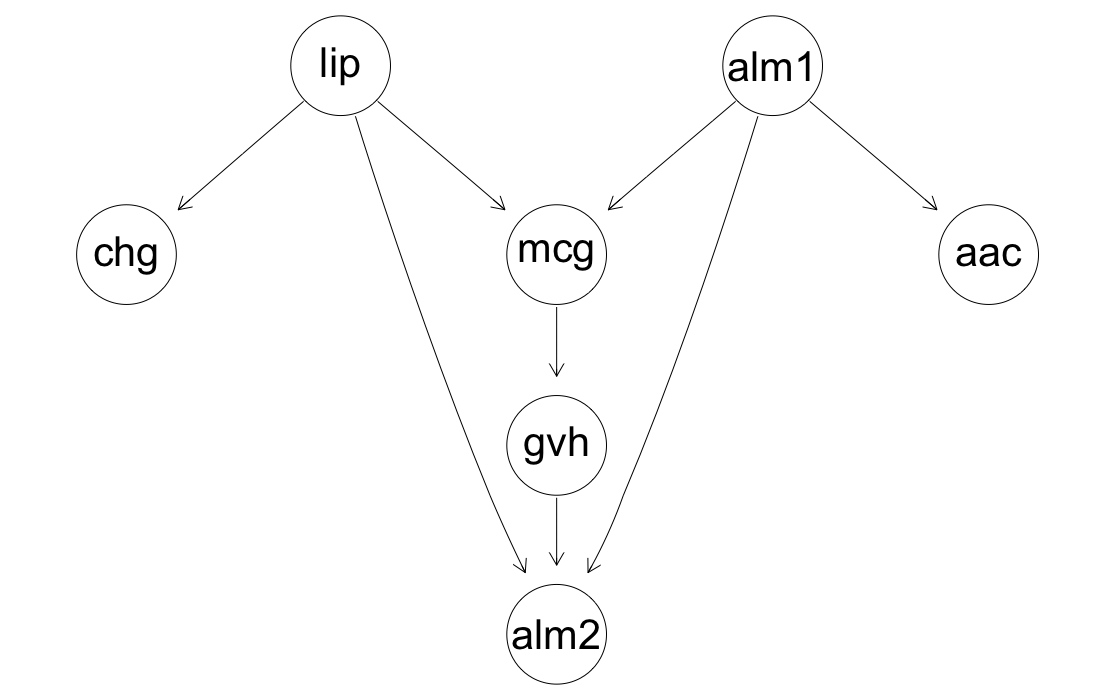
\includegraphics[width=0.6\textwidth]{FIGS/dagEcoli.png}

	\caption{Directed acyclic graph learned from 80 percent of the \code{ecoli} dataset used as training data.}
	\label{fig:dag}
\end{figure}

Before describing how to learn the MoTBF distributions associated with the network structure, we first present the basic
functionality for learning different types of MoTBF representations, i.e., univariate, conditional, and joint
MoTBF densities.

We illustrate the learning of a univariate MoTBF density by considering the continuous variable \code{mcg}.  
\begin{example}
> f1 <- univMoTBF(trainingData[,1], POTENTIAL_TYPE = "MTE", nparam = 13)
> f2 <- univMoTBF(trainingData[,1], POTENTIAL_TYPE = "MOP", nparam = 11)
\end{example}

The \code{univMoTBF()} function is used for learning univariate densities. The function is at the core of a collection of functions included in the package
to learn densities of class \code{"motbf"} from data. Least squares optimization is used
to minimize the mean squared error between the empirical cumulative distribution and the estimated MoTBF.

The function takes two mandatory arguments, \code{data} and \code{POTENTIAL\_TYPE}, where the latter can
either be \code{"MOP"} or \code{"MTE"} if polynomial or exponential basis functions should be used, respectively.
\code{univMoTBF()} also accepts optional arguments: it is possible to specify the domain over which the model will be fitted, \code{evalRange}, the exact number
of basis functions to be used, \code{nparam}, and the maximum number of parameters in the function, \code{maxParam},
which selects the best fit using the log-likelihood score. 
If \code{nparam} or \code{maxParam} are not given, then the Bayesian information criterion (BIC)
\citep{Sch78} is used for scoring and function selection: 
it evaluates the two next functions and if the BIC value does not improve then the function with the best BIC score so far is returned.

An overview of the obtained results is shown via \code{print()} and \code{summary()}.\footnote{In order to save space
and increase readability, we are only printing the 4 most significant digits in the examples in this paper.}


\begin{example}
R> print(f1)


[1] 31692.5765-19886.9389*exp(2*x)-3430.0930*exp(-2*x)+6520.8968*exp(4*x)
-91374.9603*exp(-4*x)-1269.7572*exp(6*x)+189285.9358*exp(-6*x)
+145.8260*exp(8*x)-186348.2886*exp(-8*x)-8.9962*exp(10*x)+94460.6774*exp(-10*x)
+0.2244*exp(12*x)-19787.1017*exp(-12*x)


> summary(f2)

MoTBFs FOR UNIVARIATE DISTRIBUTIONS 

Model:
0.0009+31.8820*x-1161.8247*x^2+16513.1506*x^3-121362.4662*x^4+529132.7157*x^5
-1434074.5145*x^6+2426253.6805*x^7-2482246.1917*x^8+1401057.0127*x^9-334304.5309*x^10 

Class: motbf
Subclass: mop 

Coefficients:
0.001 31.8821 -1161.825 16513.15 -121362.5 529132.7 -1434075 2426254 
-2482246 1401057 -334304.5 

Domain:
(0, 0.89)

Number of Iterations: 7 

Processing Time: 0.002254009 secs 
\end{example}

The object returned by \code{univMoTBF()} is a list containing several elements, including its mathematical expression and other hidden elements related to the learning task.
The processing time is one of the values returned by this function and it can be extracted by \code{\$Time}. 
Although the learning process is always the same for a particular data sample, the processing time can vary inasmuch as it depends on the CPU.

\begin{example}
> hist(trainingData[,1], prob = TRUE , main = "", xlab = "X")
> plot(f1, xlim = range(trainingData[,1]), col = "red", add = TRUE)
> plot(f2, xlim = range(trainingData[,1]), col = "blue", add = TRUE)
\end{example}

\begin{figure}
	\centering

	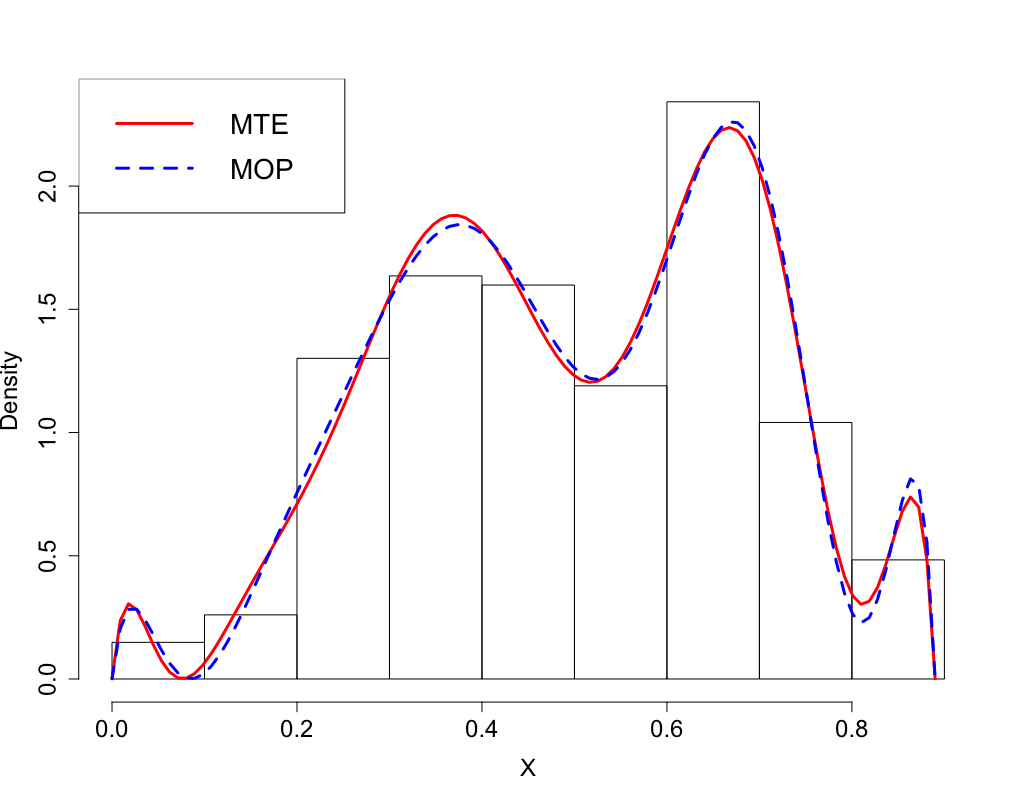
\includegraphics[width=0.6\textwidth]{FIGS/univariate.png}

	\caption{Univariate learning with blue dashed line for MOPs and red solid line for MTEs overlaying the histogram of the training data of the \code{mcg} variable.}
	\label{fig:univariate}
\end{figure}

Figure \ref{fig:univariate} shows the model fits, provided by \code{univMoTBF()}, displayed using the generic
method \code{plot()}. \\

To evaluate the predictive ability of the models  we use the generic method \code{as.function()} developed
for the \code{"motbf"} class to get the log-likelihood as well as \code{BICMoTBF()} to obtain the BIC score.

\begin{example}
> sum(log(as.function(f1)(testData[,1])))
[1] 9.1945

> sum(log(as.function(f2)(testData[,1])))
[1] 8.7249

> BICMoTBF(f1,testData[,1])
[1] -20.2383

> BICMoTBF(f2,testData[,1])
[1] -16.5032
\end{example}

An alternative way to visually check the goodness of fit of the estimated models is to simulate a data sample from 
the learned functions and compare it with the training data. For doing this, we use the inverse transform method,
a technique for generating random samples from a specific probability distribution based on evaluating the inverse of 
the CDF on a uniform random number, yielding a value for the random variable being sampled. 
This is done by function \code{rMoTBF()}.
For the sake of reproducibility, we fix the seed for the random numbers to be used by the
\code{rMoTBF()} function, which is
set to $5$ in this example. In the next code snippet, the previous function fitted with a polynomial basis, \code{f2}, will be used.

\begin{example}
> set.seed(5)
> X <- rMoTBF(size = 400, fx = f2)
> ks.test(trainingData[,1], X)

Two-sample Kolmogorov-Smirnov test

data:  trainingData[, 1] and X
D = 0.065167, p-value = 0.5018
alternative hypothesis: two-sided
\end{example}

In this example the two-sample Kolmogorov-Smirnov test is used. 
The $p$-value is notably above $0.05$, so there is no evidence to reject the null hypothesis
that both samples are drawn from the same population.

\begin{example}
> hist(X, prob = TRUE, col = "deepskyblue3", main = "", ylim = c(0,2.2))
> hist(trainingData[,1], prob = TRUE, col = adjustcolor("gold", 
+       alpha.f = 0.5), add = TRUE)
> plot(ecdf(trainingData[,1]), cex = 0, main = "")
> plot(integralMoTBF(f2), xlim = range(trainingData[,1]), col = "red", add = TRUE)
\end{example}



\begin{figure}[htb]     
	\centering
	\subcaptionbox{}{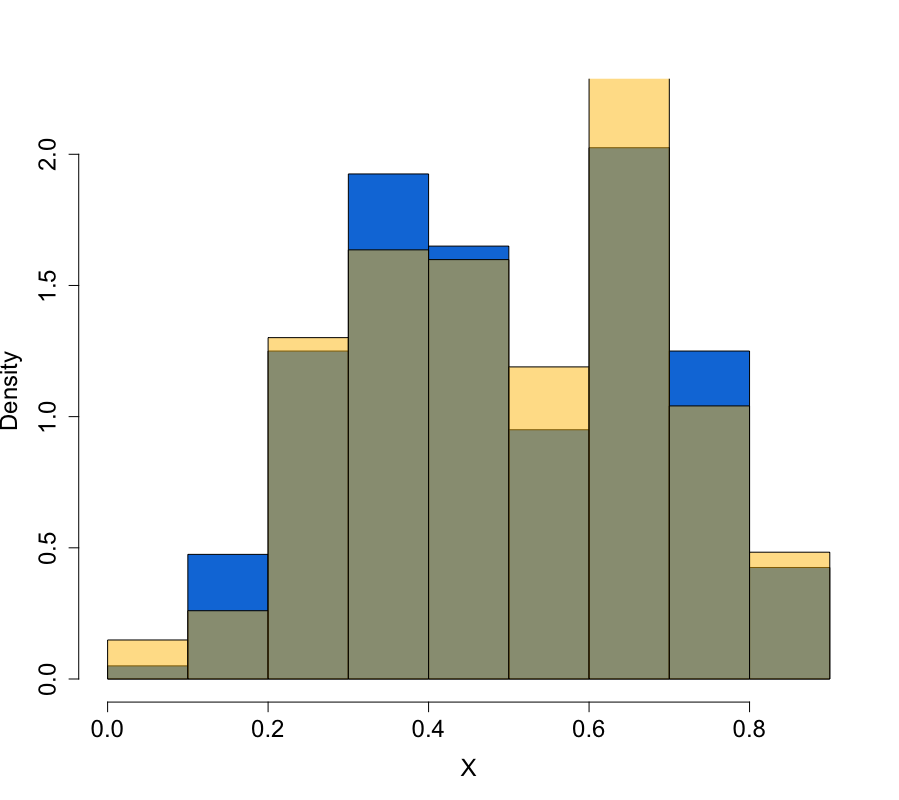
\includegraphics[width=0.495\textwidth]{FIGS/histogram.png}}
	\subcaptionbox{}{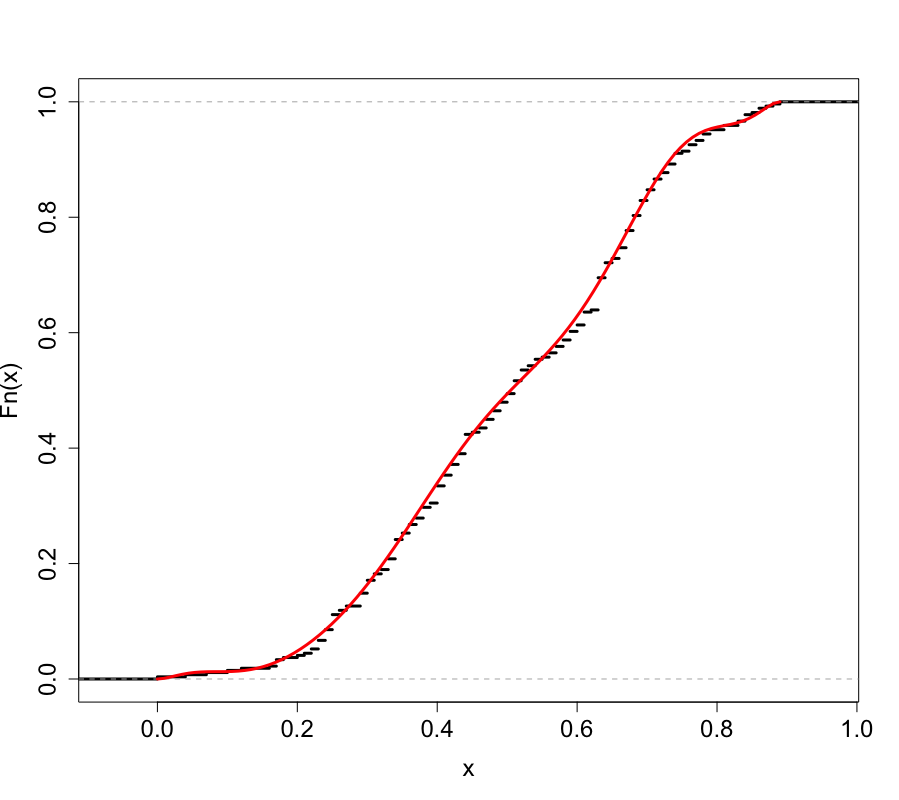
\includegraphics[width=0.495\textwidth]{FIGS/inversionMethod.png}}
	\caption{Histogram of variable \code{mcg} plotted over the histogram of the generated sample (a). 
		Illustration of the inverse transform method (b), red solid line is the CDF of the generated sample, 
		and black dashed line is the  empirical CDF of the training data for variable \code{mcg}.}
	\label{fig:randomSample}
\end{figure}

Figure~\ref{fig:randomSample} shows two plots comparing the training data of variable \code{mcg} 
and the sample simulated from the distribution learned using the same training data.

We can also manipulate the distributions with a collection of methods for class \code{"motbf"}. Here is an example of the use of three of them,
\code{coef()}, \code{integralMoTBF()}, and \code{derivMoTBF()}.

\begin{example}
> coef(f1)
[1]  3.1692e+04 -1.9886e+04 -3.4300e+03  6.5208e+03 -9.1374e+04
[6] -1.2697e+03  1.8928e+05  1.4582e+02 -1.8634e+05 -8.9962e+00
[11]  9.4460e+04  2.2449e-01 -1.9787e+04

> integralMoTBF(f2)
[1] 0.0009*x+15.9410*x^2-387.2749*x^3+4128.2876*x^4-24272.4932*x^5+88188.7859*x^6
-204867.7877*x^7+303281.7100*x^8-275805.1324*x^9+140105.7012*x^10-30391.3209*x^11

> integralMoTBF(f2, min = min(trainingData[,1]), max = max(trainingData[,1]))
[1] 1

> derivMoTBF(f2)
[1] 31.8820-2323.6495*x+49539.4519*x^2-485449.8648*x^3+2645663.5790*x^4
-8604447.0881*x^5+16983775.7655*x^6-19857969.5358*x^7+12609513.1160*x^8
-3343045.3101*x^9

\end{example}

The learning process for multidimensional variables is similar to the previous one.
The function \code{parametersJointMoTBF()} is used to solve the quadratic optimization problem. It returns
\code{Parameters}, \code{Range} and \code{Time}, among other values. The function \code{jointMoTBF()} is used
for obtaining the analytical expression, where the returned object is of class \code{"jointmotbf"}. The expression 
is the only visible element, while the others can be retrieved using \code{attributes()}.
In this example only two variables are used, \code{mcg} and \code{alm1}, in order to be able to plot the results. 

\begin{example}
> parameters <- parametersJointMoTBF(X = trainingData[,c("mcg", "alm1")],
+                dimensions = c(5,5))
> P <- jointMoTBF(parameters)
> attributes(P)

$names
[1] "Function"   "Domain"     "Iterations" "Time"      
$class
[1] "jointmotbf"
\end{example}

\begin{example}
> plot(P, data = trainingData[,c(1,6)])
> plot(P, data = trainingData[,c(1,6)], filled = FALSE)
> plot(P, type = "perspective", data = trainingData[,c(1,6)], orientation=c(60,20))
\end{example}




\begin{figure}[htb]     
	\centering
	\subcaptionbox{}{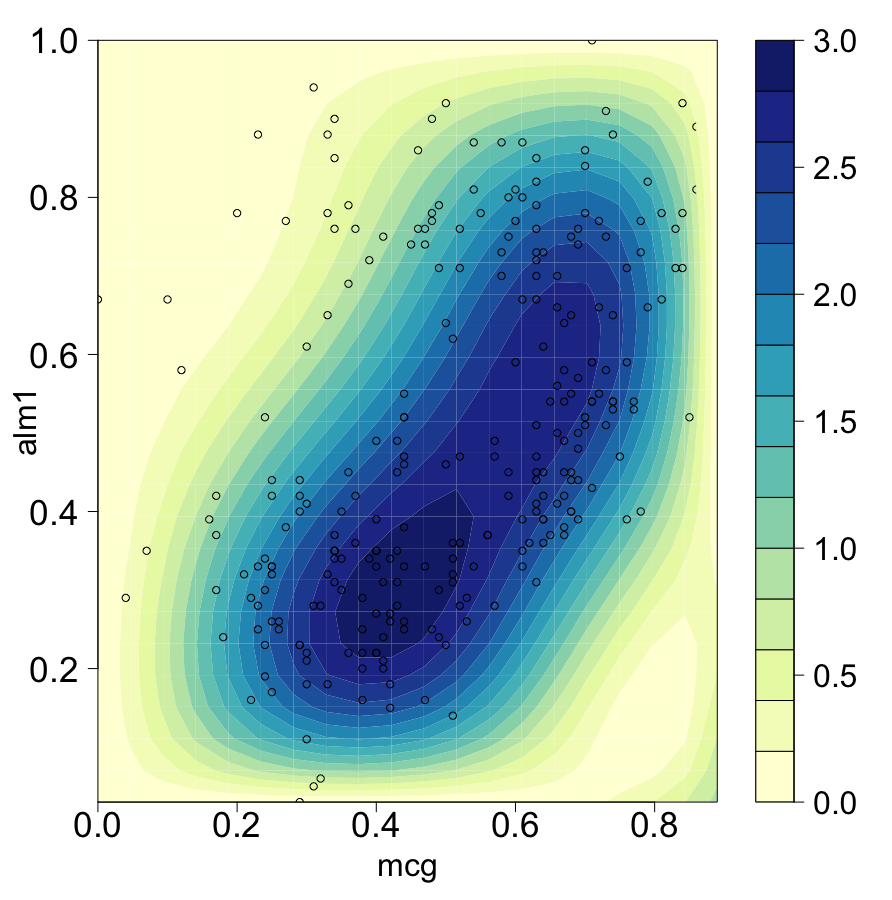
\includegraphics[width=0.33\textwidth]{FIGS/joint.png}}
	\subcaptionbox{}{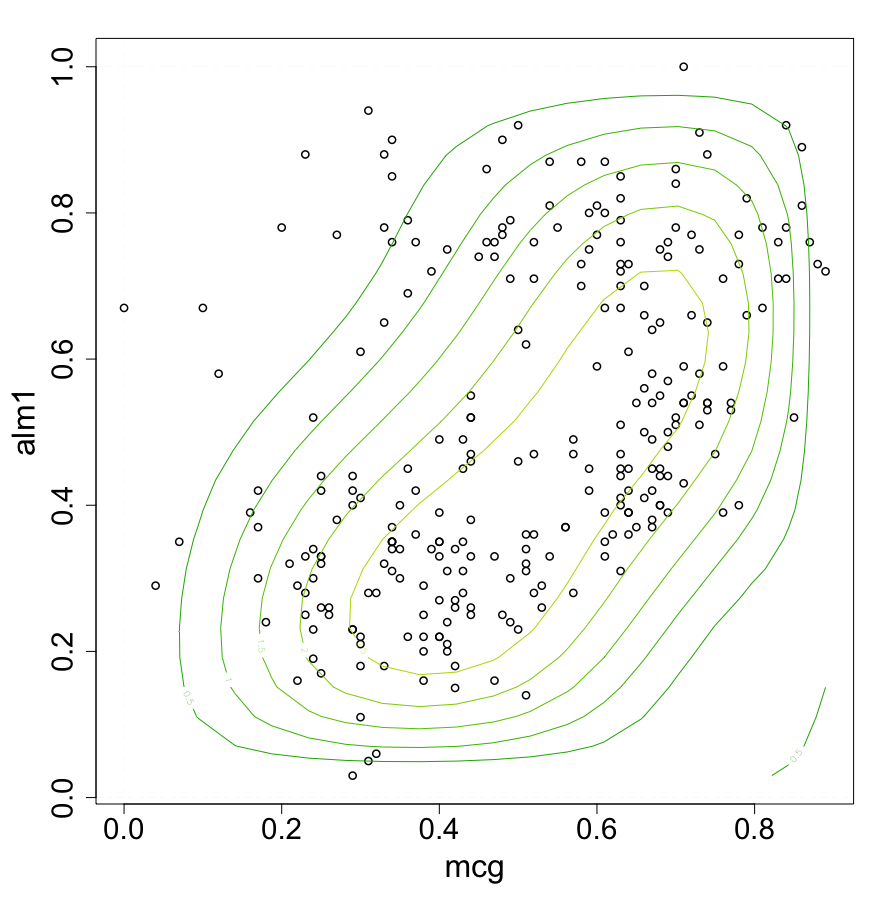
\includegraphics[width=0.33\textwidth]{FIGS/jointContour.png}}
	\subcaptionbox{}{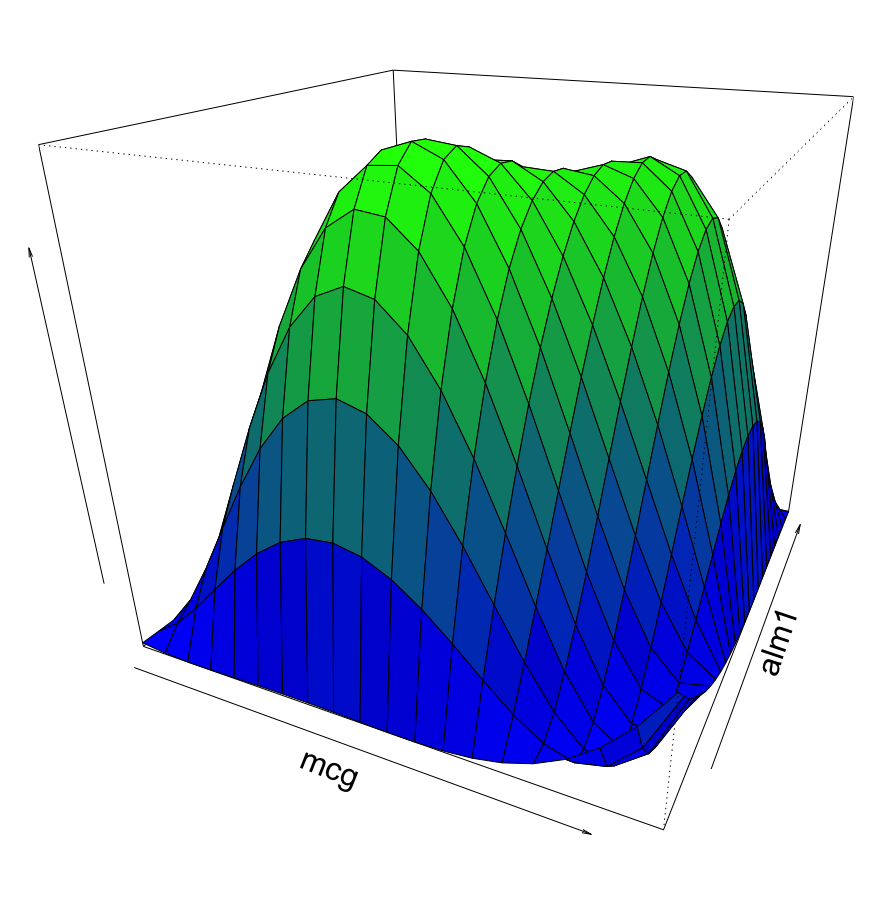
\includegraphics[width=0.32\textwidth]{FIGS/jointPersp.png}}
	\caption{Filled contour (a), simple contour (b) and perspective (c) plots of the joint MoTBF $f(Y,X)$ of variables \code{mcg} and \code{alm1}.}
	\label{fig:joint}
\end{figure}

The plots in Figure~\ref{fig:joint} are generated using \code{plot()}, developed for objects of class 
\code{"jointmotbf"}. This function accepts optional arguments such as \code{type}, where one can choose between 
\code{"perspective"} and \code{"contour"}, \code{ranges}, used to specify the plotting range, \code{orientation}, which 
indicates the orientation of the perspective graph, and \code{filled} for getting a filled contour plot.

The function \code{print()} can be used to obtain an expression of the learned joint density, while 
\code{summary()} yields a more thorough excerpt of the \code{"jointmotbf"} object.


\begin{example}
> summary(P)

MoTBFs FOR MULTIVARIATE DISTRIBUTIONS 

Model:
0.0355-0.2915*y+0.8351*y^2-0.9711*y^3+0.3939*y^4-2.9706*x+88.6144*x*y
-339.2388*x*y^2+451.7559*x*y^3-198.1810*x*y^4-9.2802*x^2+494.5320*x^2*y
-1392.3658*x^2*y^2+1175.9828*x^2*y^3-268.7925*x^2*y^4+35.3166*x^3
-1708.9509*x^3*y+5662.3268*x^3*y^2-5878.6313*x^3*y^3+1889.8292*x^3*y^4
-22.2566*x^4+1164.5531*x^4*y-4117.2185*x^4*y^2+4479.3097*x^4*y^3-1504.3348*x^4*y^4 

Class: jointmotbf 

Coefficients:
0.0355 -0.2915 0.8351 -0.9711 0.3939 -2.9706 88.6144 -339.2388 451.7559 
-198.1811 -9.2802 494.5321 -1392.366 1175.983 -268.7926 35.3166 -1708.951 
5662.327 -5878.631 1889.829 -22.2566 1164.553 -4117.219 4479.31 -1504.335 

Domain x:
(0, 0.89)
Domain y:
(0.03, 1)

Number of Iterations: 96 

Processing Time: 1.144651 secs 
\end{example}

As in the univariate case, the processing time, \code{P\$Time}, can vary depending on the CPU, but the
learning outcome will always be  the same for a specific data sample.
 The \code{marginalJointMoTBF()} function computes the marginals of joint densities.
In this example we have two variables, so there are two marginal densities.

\begin{example}
> marginalJointMoTBF(P, var = 1)
[1] 0.0031+1.6119*x+14.1692*x^2-23.7487*x^3+6.7540*x^4

> marginalJointMoTBF(P, var = 2)
[1] -0.2716+13.0463*y-32.4520*y^2+32.5558*y^3-12.8781*y^4
\end{example}


The next step in our analysis is learning conditional densities,  which is implemented by the function 
\code{conditionalMethod()}.
Five of its arguments are compulsory:  \code{data}, the dataset; \code{nameParents}, a character
vector indicating the name of the parents; \code{nameChild}, a character string containing the name of
the child; \code{numIntervals}, the maximum number of intervals for splitting the domain of the parent
variables; \code{POTENTIAL\_TYPE},  the type of basis function. Other arguments are optional,
like \code{maxParam}, indicating the maximum number of parameters for each function, and \code{s}, the
expert's relative confidence in any prior knowledge, and 
\code{priorData} if prior knowledge is incorporated in the analysis. 

We will do the conditional analysis for only two variables in order to be able to make a 2-dimensional plot of
the obtained results using \code{plotConditional()}. For example, taking into account the relationship found
by the dag, we consider the child variable \code{gvh} with parent variable \code{mcg}.

\begin{example}
> P <- conditionalMethod(trainingData, nameParents = "mcg", nameChild = "gvh",
+       numIntervals = 5, POTENTIAL_TYPE ="MOP")
> printConditional(P)

Parent: mcg    	 Range: 0 < mcg < 0.44 
[1] 115.8704-1783.8943*x+10688.6518*x^2-32342.1750*x^3+54497.1689*x^4-52033.2599*x^5
+26393.6470*x^6-5536.0079*x^7
Parent: mcg    	 Range: 0.44 < mcg < 0.89 
[1] -37.3009+733.0877*x-5676.3802*x^2+22283.2874*x^3-47834.5916*x^4+56908.0376*x^5
-35242.7482*x^6+8867.5576*x^7
\end{example}


\begin{example}
> plotConditional(P, data = trainingData, nameChild = "gvh", points = TRUE)
\end{example}

\begin{figure}
	\centering

	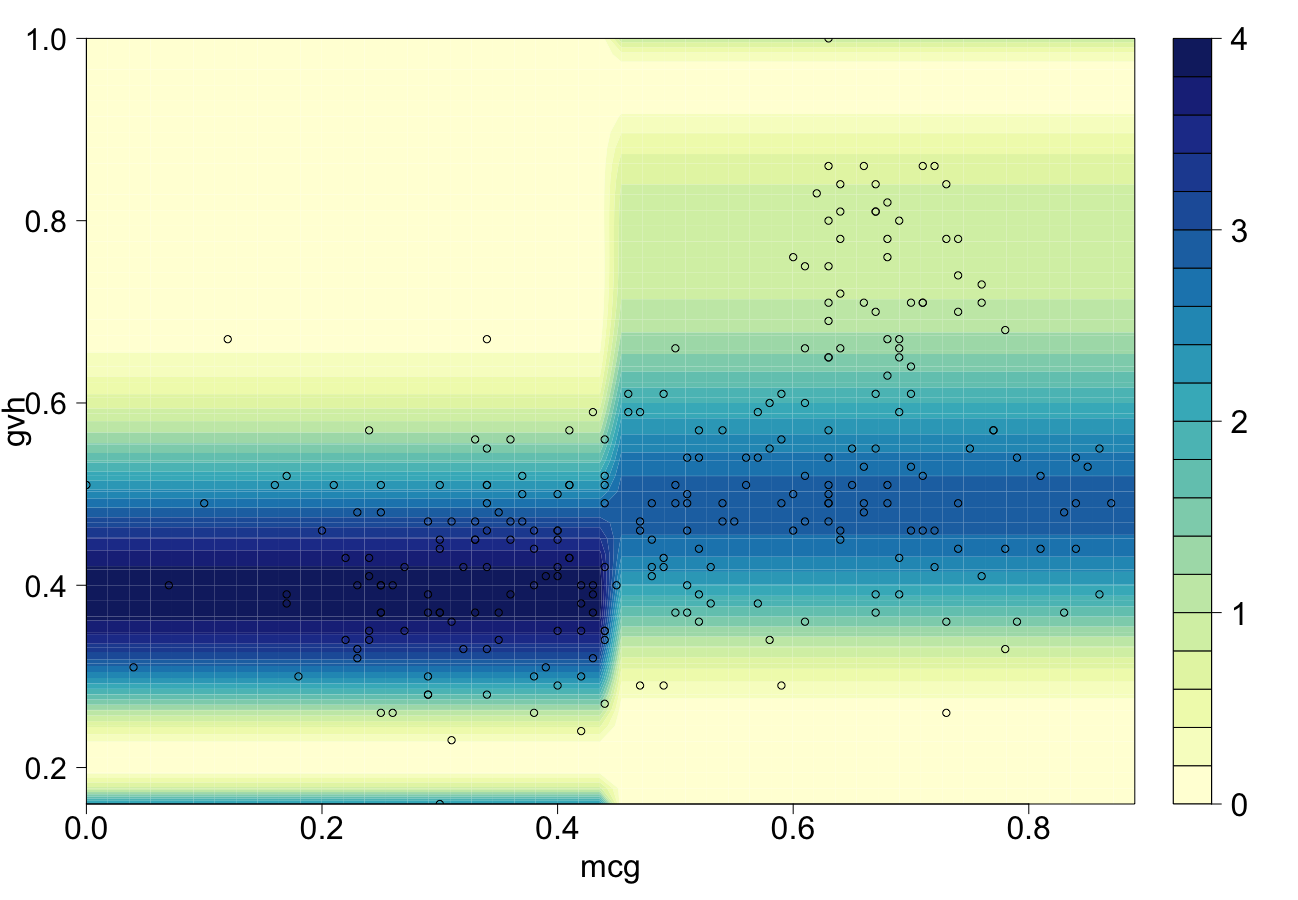
\includegraphics[width=0.6\textwidth]{FIGS/conditional.png}

	\caption{Conditional density of \code{gvh} given \code{mcg}.}
	\label{fig:conditional}
\end{figure}

Figure~\ref{fig:conditional} shows the resulting conditional density (a MOP in this case) with the sample points overlaid.
It can be noticed that the learning algorithm decides to split the domain of the parent into two intervals 
even though we have set the argument \code{numIntervals} to five. This is because the BIC score is not
improved any further by splitting the domain into more than two intervals. 

The last step is to learn the distributions tied to the Bayesian network learned previously.
For doing this task, the \code{MoTBFs\_Learning()} function of the \pkg{MoTBFs} package is used.
The graph is a mandatory argument, that can be of class \code{"bn"}, \code{"graphNEL"} or \code{"network"}.
Other mandatory arguments are the \code{data}, the maximum number of intervals for splitting the domain of the parents, 
 and the type of basis function. The function also accepts additional arguments, but they are not listed here.

In the example, the DAG was obtained using the \pkg{bnlearn} package and therefore it is
an object of class \code{"bn"}. As an example, 
we will use a maximum of $4$ intervals and \code{"MTE"} potentials when learning the densities (i.e. exponential
basis functions).


\begin{example}
> bn <- MoTBFs_Learning(dag, data = trainingData, numIntervals = 4,
+        POTENTIAL_TYPE = "MTE")
> printBN(bn)

Potential(mcg)
Parent: alm1    	 Range: 0.03 < alm1 < 0.33 
Parent: lip    	 Range = "0.48" 
[1] 77.3522-39.7786*exp(2*x)-4.7525*exp(-2*x)+7.4896*exp(4*x)
-110.4468*exp(-4*x)-0.48548*exp(6*x)+71.3407*exp(-6*x)
Parent: alm1    	 Range: 0.33 < alm1 < 1 
Parent: lip    	 Range = "0.48" 
[1] -5.4620+3.3347*exp(2*x)+3.6655*exp(-2*x)-0.4237*exp(4*x)-1.0852*exp(-4*x)
Parent: lip    	 Range = "1" 
[1] -11.4070+6.0014*exp(2*x)+4.4488*exp(-2*x)-0.7109*exp(4*x)+2.3944*exp(-4*x)

Potential(gvh)
Parent: mcg    	 Range: 0 < mcg < 0.51 
[1] -97.6780+34.1822*exp(2*x)-282.2167*exp(-2*x)-2.7274*exp(4*x)+2028.8986*exp(-4*x)
-0.12096*exp(6*x)-3609.5088*exp(-6*x)+0.0175*exp(8*x)+2069.4440*exp(-8*x)
Parent: mcg    	 Range: 0.51 < mcg < 0.89 
[1] 685.6507-360.2896*exp(2*x)+252.1477*exp(-2*x)+79.5432*exp(4*x)-3074.9108*exp(-4*x)
-8.3530*exp(6*x)+4377.0877*exp(-6*x)+0.3410*exp(8*x)-2004.8518*exp(-8*x)

Potential(lip)
0.9630 0.0369


Potential(chg)
Parent: lip    	 Range = "0.48" 
1 0 
Parent: lip    	 Range = "1" 
0.8181 0.1818 


Potential(aac)
Parent: alm1    	 Range: 0.03 < alm1 < 1 
[1] -3742.3665+2528.6429*exp(2*x)+1860.6477*exp(-2*x)-894.0268*exp(4*x)
+2121.1450*exp(-4*x)+175.4771*exp(6*x)-3473.1126*exp(-6*x)-18.0836*exp(8*x)
+1679.6126*exp(-8*x)+0.7634*exp(10*x)-238.3277*exp(-10*x)

Potential(alm1)
[1] 158.6127-95.2652*exp(2*x)-56.9318*exp(-2*x)+25.4631*exp(4*x)-97.0824*exp(-4*x)
-3.1624*exp(6*x)+52.8052*exp(-6*x)+0.1480*exp(8*x)+17.6287*exp(-8*x)

Potential(alm2)
Parent: alm1    	 Range: 0.03 < alm1 < 0.33 
Parent: gvh    	 Range: 0.16 < gvh < 1 
Parent: lip    	 Range = "0.48" 
[1] 193.4903-112.6569*exp(2*x)-52.9058*exp(-2*x)+28.5291*exp(4*x)-185.8167*exp(-4*x)
-3.3698*exp(6*x)+155.0492*exp(-6*x)+0.1517*exp(8*x)-21.3863*exp(-8*x)
Parent: alm1    	 Range: 0.33 < alm1 < 0.45 
Parent: gvh    	 Range: 0.16 < gvh < 1 
Parent: lip    	 Range = "0.48" 
[1] 395.0603-217.7061*exp(2*x)+16.0642*exp(-2*x)+51.0248*exp(4*x)-1009.4114*exp(-4*x)
-5.6246*exp(6*x)+1224.5254*exp(-6*x)+0.2387*exp(8*x)-454.1703*exp(-8*x)
Parent: alm1    	 Range: 0.45 < alm1 < 0.71 
Parent: gvh    	 Range: 0.16 < gvh < 1 
Parent: lip    	 Range = "0.48" 
[1] -3.0260+3.1097*exp(2*x)+6.9062*exp(-2*x)-0.8013*exp(4*x)-12.5762*exp(-4*x)
+0.0578*exp(6*x)+6.3306*exp(-6*x)
Parent: lip    	 Range = "1" 
[1] 1.9648-0.2660*exp(2*x)-0.2660*exp(-2*x)
Parent: alm1    	 Range: 0.71 < alm1 < 1 
Parent: gvh    	 Range: 0.16 < gvh < 1 
Parent: lip    	 Range = "0.48" 
[1] -1.2697+0.6353*exp(2*x)+0.6353*exp(-2*x)
Parent: lip    	 Range = "1" 
[1] 1.0101+0*exp(2*x)
\end{example}

The results are reported using the \code{printBN()} function. Notice how nodes in the DAG with only
discrete parents contain as many functions as configurations of the parents, nodes that have continuous parents have 
at most $4$ functions for each parent and nodes that have mixed parents contain as many functions as
configurations of the discrete parents times the number of regions into which the domain of the continuous
parents is split. The BIC criterion is used to decide the number of splitting points of the domain of the continuous parent 
nodes and to choose the number of basis functions used.
The function \code{BiC.MoTBFBN()} can be used to compute the log-likelihood and the BIC score of a dataset
given the Bayesian network.

\begin{example}
> bic <- BiC.MoTBFBN(bn, data = testData)
> attributes(bic)
$names
[1] "LogLikelihood" "BIC" 

> bic$LogLikelihood
[1] 173.5496
> bic$BIC
[1] -51.40147
\end{example}
		
		
We will now exemplify the use of prior knowledge in the learning process.
In order to illustrate the approach, we first select a small subset of the \code{Ecoli} dataset using
\code{TrainingandTestData()}. In the next example the percentage of the test data is $99\%$, which means the training data is only $1\%$ of the full dataset.
		
\begin{example}
> set.seed(4)
> dataTT <- TrainingandTestData(data, percentage_test = 0.99)
> trainingData <- dataTT$Training
> testData <- dataTT$Test
> nrow(trainingData)
[1] 13
\end{example}
		
		There are $13$ entries in the training dataset. We are going to fit MoTBFs with and without prior information.
		To generate an artificial prior dataset the \code{generateNormalPriorData()} function can be used.
		
\begin{example}
> means <-  sapply(data, mean)
> set.seed(4)
> priorData <- generateNormalPriorData(dag, data = trainingData, size = 5000, 
+               means = means)
\end{example}
		
Learning univariate and conditional distributions and Bayesian networks can be done using the functions
\code{learnMoTBFpriorInformation()} and \code{MoTBFs\_Learning()}. The arguments for these functions are 
the same as previously  explained and, in addition, it is necessary to specify the expert confidence in the prior 
knowledge, \code{s}, and the prior dataset \code{priorData}. Argument $s$ takes values on the interval $[0,N]$, 
where $N$ is the sample size, and is used to synchronize the support of the prior knowledge and the sample. 
We refer the reader to \citep{Per15} for the details. In this example we will use the \code{aac} variable from the 
data set, have \code{s = 5} as confidence level, and set \code{"MOP"} as potential type.
		
\begin{example}
> f <- learnMoTBFpriorInformation(priorData$aac, trainingData$aac,
+	s = 5, POTENTIAL_TYPE = "MOP")
> attributes(f)

$names
[1] "coeffs"            "posteriorFunction" "priorFunction"    
[4] "dataFunction"      "domain"  

> print(f)

$coeffs
[1] 0.5509206 0.4490794

$posteriorFunction
[1] 0.2911+2.7626*x+4.3721*x^2-30.4218*x^3-0.8389*x^4+965.8444*x^5-4183.3860*x^6
+7735.8433*x^7-7321.9450*x^8+3498.9449*x^9-671.5104*x^10

$priorFunction
[1] 0.0673+1.7639*x+11.8532*x^2-55.2199*x^3-1.5228*x^4+1753.1465*x^5-7593.4470*x^6
+14041.6676*x^7-13290.3826*x^8+6351.0879*x^9-1218.8879*x^10

$dataFunction
[1] 0.5656+3.9878*x-4.8055*x^2

$domain
[1] -0.1232  0.9531

\end{example}
				
\begin{example}
> sum(log(as.function(f$posteriorFunction)(testData$aac)))
[1] 134.566
> sum(log(as.function(f$dataFunction)(testData$aac)))
[1] 78.96405
\end{example}

The best model, taking into account the log-likelihood, is the MoTBF which uses the prior data, \code{f\$posteriorFunction}.
The generic method \code{plot()} for \code{"motbf"} object is used for displaying the functions depicted
in Figure~\ref{fig:priorUniv}.

\begin{example}
> plot(f$posteriorFunction, xlim = f$domain, ylim = c(0,2.1))
> plot(f$dataFunction, xlim = f$domain, add = TRUE, col = 2)
> plot(f$priorFunction, xlim = f$domain, add = TRUE, col = 4)
\end{example}
				
				
				
\begin{figure}
	\centering

	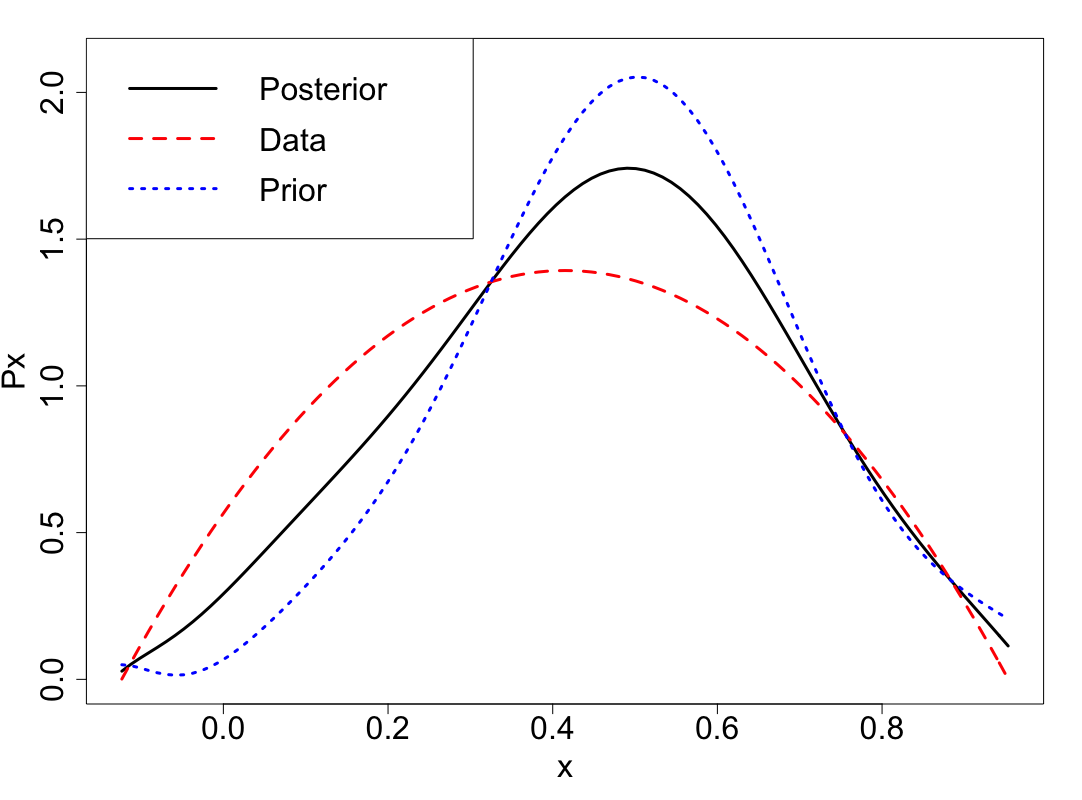
\includegraphics[width=0.6\textwidth]{FIGS/priorUnivariate.png}

	\caption{Univariate density estimation using prior knowledge. Solid black, dashed red and dotted blue lines represent the posterior, the data, and the prior function, respectively.}
	\label{fig:priorUniv}
\end{figure}

The last step is to incorporate the prior knowledge in the full Bayesian network. For this analysis we are not going to print 
out the results, because the structure is similar to the previous Bayesian network representations. As an example, we will use 
\code{numIntervals = 2}, \code{POTENTIAL\_TYPE = "MOP"}, and \code{s = 5}.

\begin{example}
> priorBN <- MoTBFs_Learning(dag, trainingData, numIntervals = 2, 
+             POTENTIAL_TYPE = "MOP", s = 5, priorData = priorData)
> BN <- MoTBFs_Learning(dag, trainingData, numIntervals = 2, POTENTIAL_TYPE = "MOP")

> logLikelihood.MoTBFBN(priorBN, data = testData)
[1] 124.384
> logLikelihood.MoTBFBN(BN, data = testData) 
[1] 14.64589
\end{example}

Looking at the log-likelihood corresponding to the network with and without prior data, we can see that,
in this example, incorporating prior knowledge is better when data is scarce.

After a Bayesian network has been constructed, the \pkg{MoTBFs} package can be used to obtain the conditional 
density of any variable  in the network given that some other variables have been observed. The conditional 
distribution is obtained by forward sampling. As an example, consider a network estimated from the \code{ecoli} dataset:

\begin{example}
> data("ecoli", package = "MoTBFs")
> data <- ecoli[,-c(1,9)]
> dag <- LearningHC(data)
> bn <- MoTBFs_Learning(dag, data = data, numIntervals = 4, POTENTIAL_TYPE = "MTE")
\end{example}
The observed values are specified using a data frame. In the example, we are assuming that we want to compute
the conditional density of \code{alm2} given that \code{lip="0.48"}, \code{alm1 = 0.55} and \code{gvh = 1}.
This is achieved by using the function \code{forward\_sampling} were we have chosen a sample size equal to 10 specified
by parameter \code{size = 10}.

\begin{example}
> obs <- data.frame(lip = "0.48", alm1 = 0.55, gvh = 1, stringsAsFactors=FALSE)
> node <- "alm2"
> set.seed(5)
> forward_sampling(bn, dag, target = node, evi = obs, size = 10, maxParam = 15)

Processing Time: 0.209545850753784secs

$fx
[1] -4.3738+2.4552*exp(2*x)+1.5054*exp(-2*x)-0.2392*exp(4*x)+2.0045*exp(-4*x)

$sample
mcg gvh  lip chg       aac alm1       alm2
1  0.7450156   1 0.48 0.5 0.3564026 0.55 0.53709571
2  0.2493266   1 0.48 0.5 0.4873396 0.55 0.55395502
3  0.4075408   1 0.48 0.5 0.5052861 0.55 0.74832025
4  0.3205169   1 0.48 0.5 0.4844040 0.55 0.82546475
5  0.4448844   1 0.48 0.5 0.4248584 0.55 0.07672959
6  0.5717975   1 0.48 0.5 0.4611889 0.55 0.35412707
7  0.7548104   1 0.48 0.5 0.5695499 0.55 0.68322911
8  0.5475842   1 0.48 0.5 0.7797320 0.55 0.45343460
9  0.3048408   1 0.48 0.5 0.5251502 0.55 0.73064241
10 0.7281756   1 0.48 0.5 0.3819332 0.55 0.70396470

\end{example}
		
The output consists of the posterior density and the sample from which the density parameters were estimated.
						
						

\section{Conclusions}
\label{sec:conclusions}
This paper has presented the R package \pkg{MoTBFs} for learning Mixtures of Truncated Basis Functions in hybrid Bayesian networks.
It provides a free and accessible implementation of algorithms for learning the parameters of MoTBFs densities as
well as MoTBF-based Bayesian networks relying on state-of-the-art learning algorithms.

The \pkg{MoTBFs} package is designed to provide the required implementation to tackle experimental data analysis 
with both discrete and continuous data. Not only does the package provide methods for learning distributions from data, 
it also includes a set of auxiliary functions to perform descriptive statistics 
as well as other basic operations like inference using forward sampling.

The \pkg{MoTBFs} package expands the functionality for handling hybrid Bayesian networks already provided by 
packages \pkg{bnlearn} and \pkg{HydeNet}, by implementing MoTBF distributions, resulting in unrestricted
network structures, regardless of the discrete or continuous nature of the variables involved, and by providing 
methods for building models from data that are compatible with exact inference methods. The package
\pkg{MoTBFs} is complementary to \pkg{abn} in the sense that the former is based on MoTBF densities, which 
do not belong to the exponential family.

\section{Acknowledgments}
This research has been partly funded by the Spanish Ministry of Science and Innovation,
through projects TIN2016-77902-C3-3-P, PID2019-106758GB-C32 and by ERDF-FEDER funds.

\bibliography{maldonado}

\address{Inmaculada Pérez-Bernabé\\
  Department of Mathematics\\
  University of Almer\'ia\\
  Almería, 04120, Spain\\
%  (ORCiD if desired)\\
  \email{iperez@ual.es}}

\address{Ana D. Maldonado\\
  Department of Mathematics\\
  University of Almer\'ia\\
  Almería, 04120, Spain\\
  (ORCiD: 0000-0001-8253-2526)\\
  \email{ana.d.maldonado@ual.es}}

\address{Thomas D. Nielsen\\
  Department of Computer Science\\
   Aalborg University\\
  Aalborg, 9220, Denmark\\
%  (ORCiD if desired)\\
  \email{tdn@cs.aau.dk}}

\address{Antonio Salmerón\\
	Department of Mathematics and \\
	Center for the Development and Transfer of Mathematical Research to Industry (CDTIME)\\
	University of Almer\'ia\\
	Almería, 04120, Spain\\
	(ORCiD: 0000-0003-4982-8725)\\
	\email{antonio.salmeron@ual.es}}

\end{article}

\end{document}
